%%%%%%%%%%%%%%%%%%%%%%%%%%%%%%%%%%%%%%%%%%%%%%%%%%%%%%%%%%%%%%%%%%% 
%% Introduccion y desarrollo del algoritmo
%%%%%%%%%%%%%%%%%%%%%%%%%%%%%%%%%%%%%%%%%%%%%%%%%%%%%%%%%%%%%%%%%%%


\section{Introducci\'on}
\begin{frame}
  \frametitle{\textbf{Tabla de Contenidos}}
  \begin{center}
    {\vspace{-1.5cm}\Large \textbf{Sección \thesection}\vspace{0.5cm}}
    \begin{beamercolorbox}[
      sep=8pt,center]{part title}
      \usebeamerfont{part title}
      \textbf{\insertsection}
    \end{beamercolorbox}
  \end{center}
\end{frame}


\begin{frame}
  \frametitle{\textbf{Introducción}}
   \begin{block}{\centering \textbf{Objetivos y alcances}}
    \begin{itemize} %\justifying\footnotesize
        \item Se desea modificar la probabilidad de ocurrencia de cada símbolo en una   transmisión digital, cambiando así la forma de su constelación. Esto se conoce como `Probabilistic Shaping'. 
        \item Para esto se utilizará el método `Distribution Matching', el cual permite transformar una secuencia de entrada, con distribución uniforme, a una secuencia de salida con una distribución diferente. 
        \item Se simulará e implementará el algoritmo en una FPGA y se analizarán los resultados obtenidos.
    \end{itemize}
    \end{block}
    \vspace{-0.2cm}
    \begin{figure}[!t] \centering
    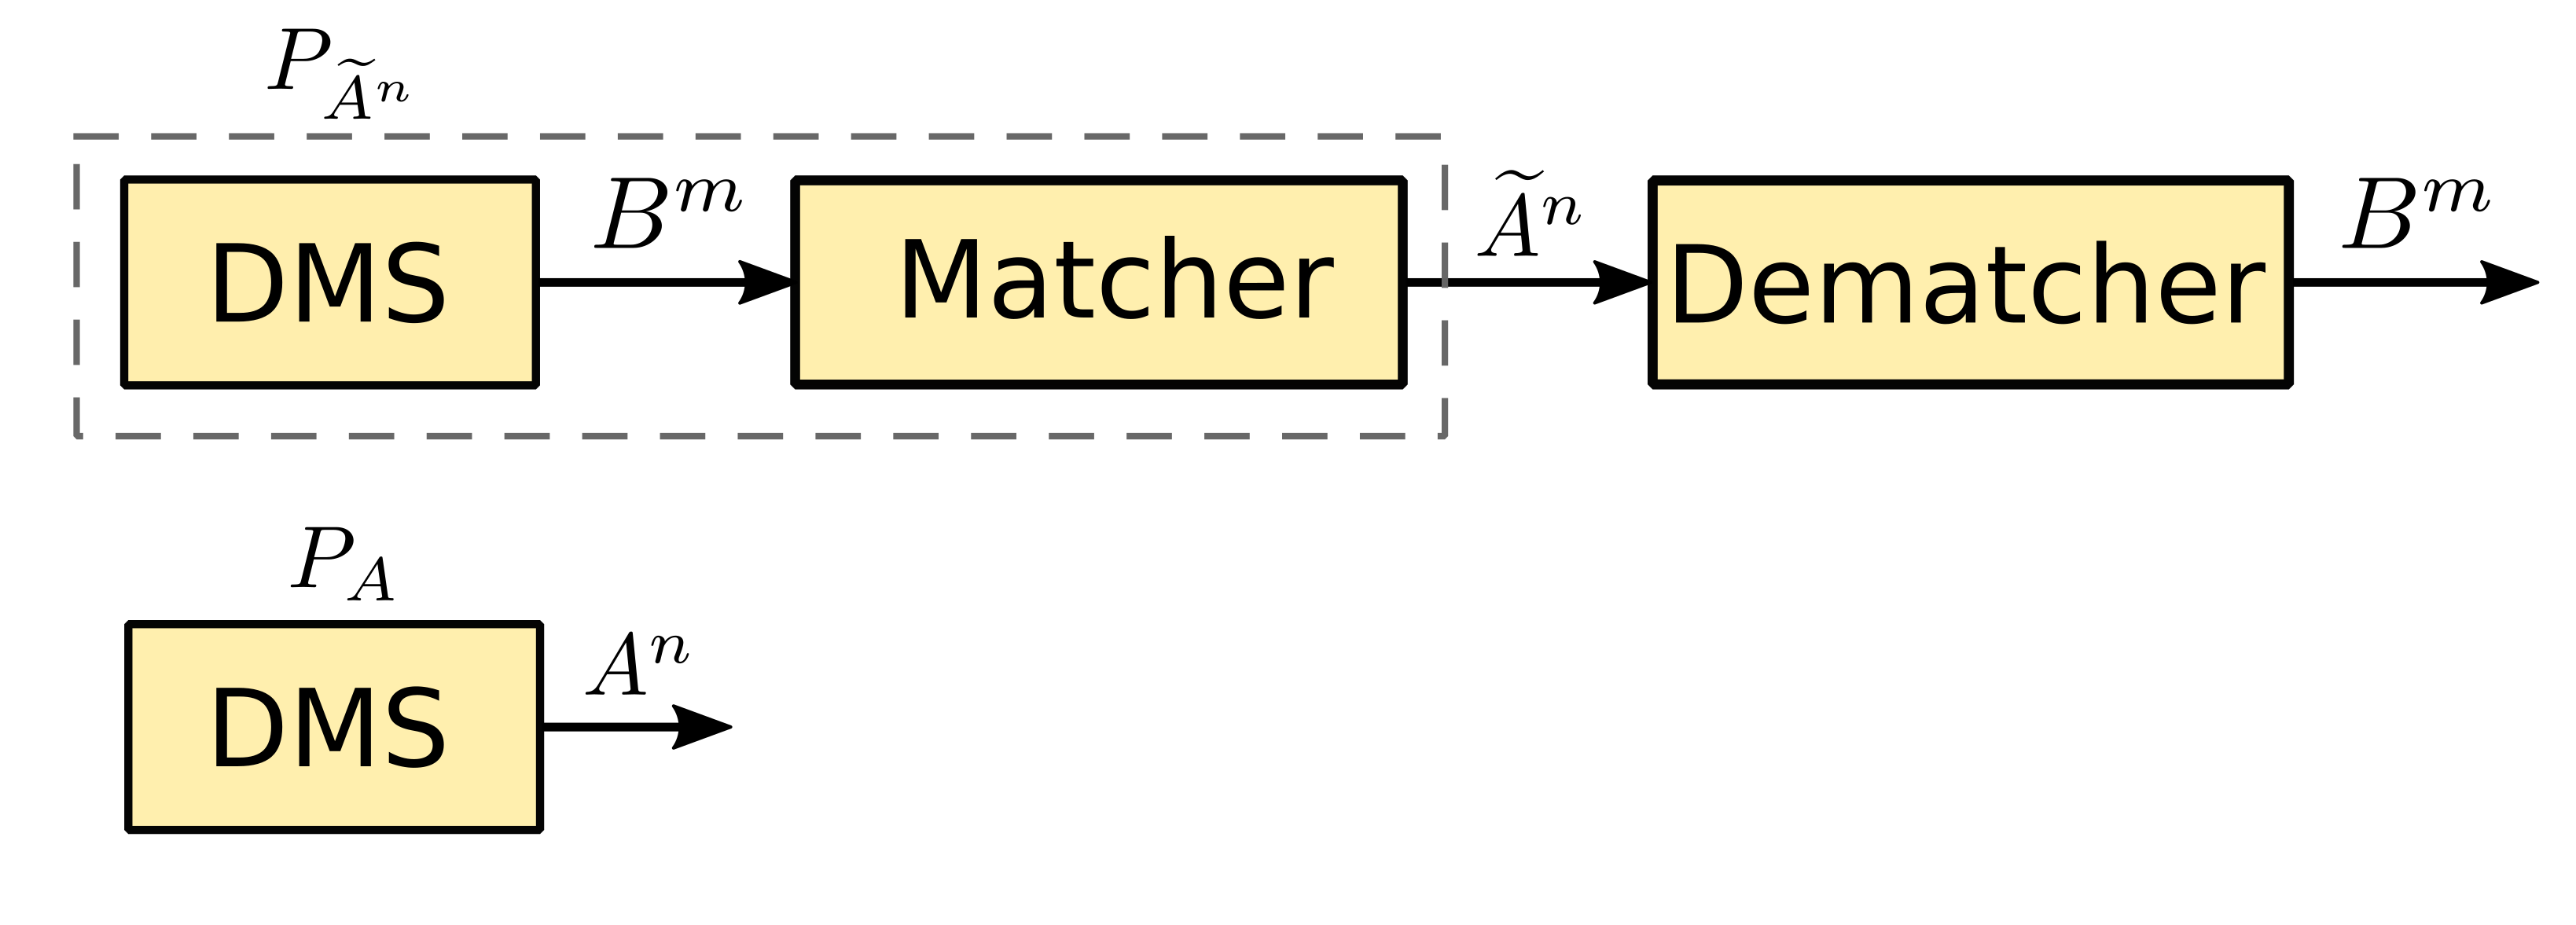
\includegraphics[width=0.70\paperwidth]{Diagramas/matcher.png}
    \end{figure}
\end{frame}


\section{Desarrollo}
\subsection{Investigación}

\begin{frame}
  \frametitle{\textbf{Tabla de Contenidos}}
  \begin{center}
    {\vspace{-1.5cm}\Large \textbf{Sección \thesection: \secname }\vspace{0.5cm}}
    \begin{beamercolorbox}[
      sep=8pt,center]{part title}
      \usebeamerfont{part title}
      \textbf{\subsecname}
    \end{beamercolorbox}
  \end{center}
\end{frame}


\begin{frame}
  \frametitle{\textbf{Flujo de trabajo}}
      \framesubtitle{\secname : \subsecname}

  \vspace{-0.3cm}
  \begin{figure}[!t] \centering
  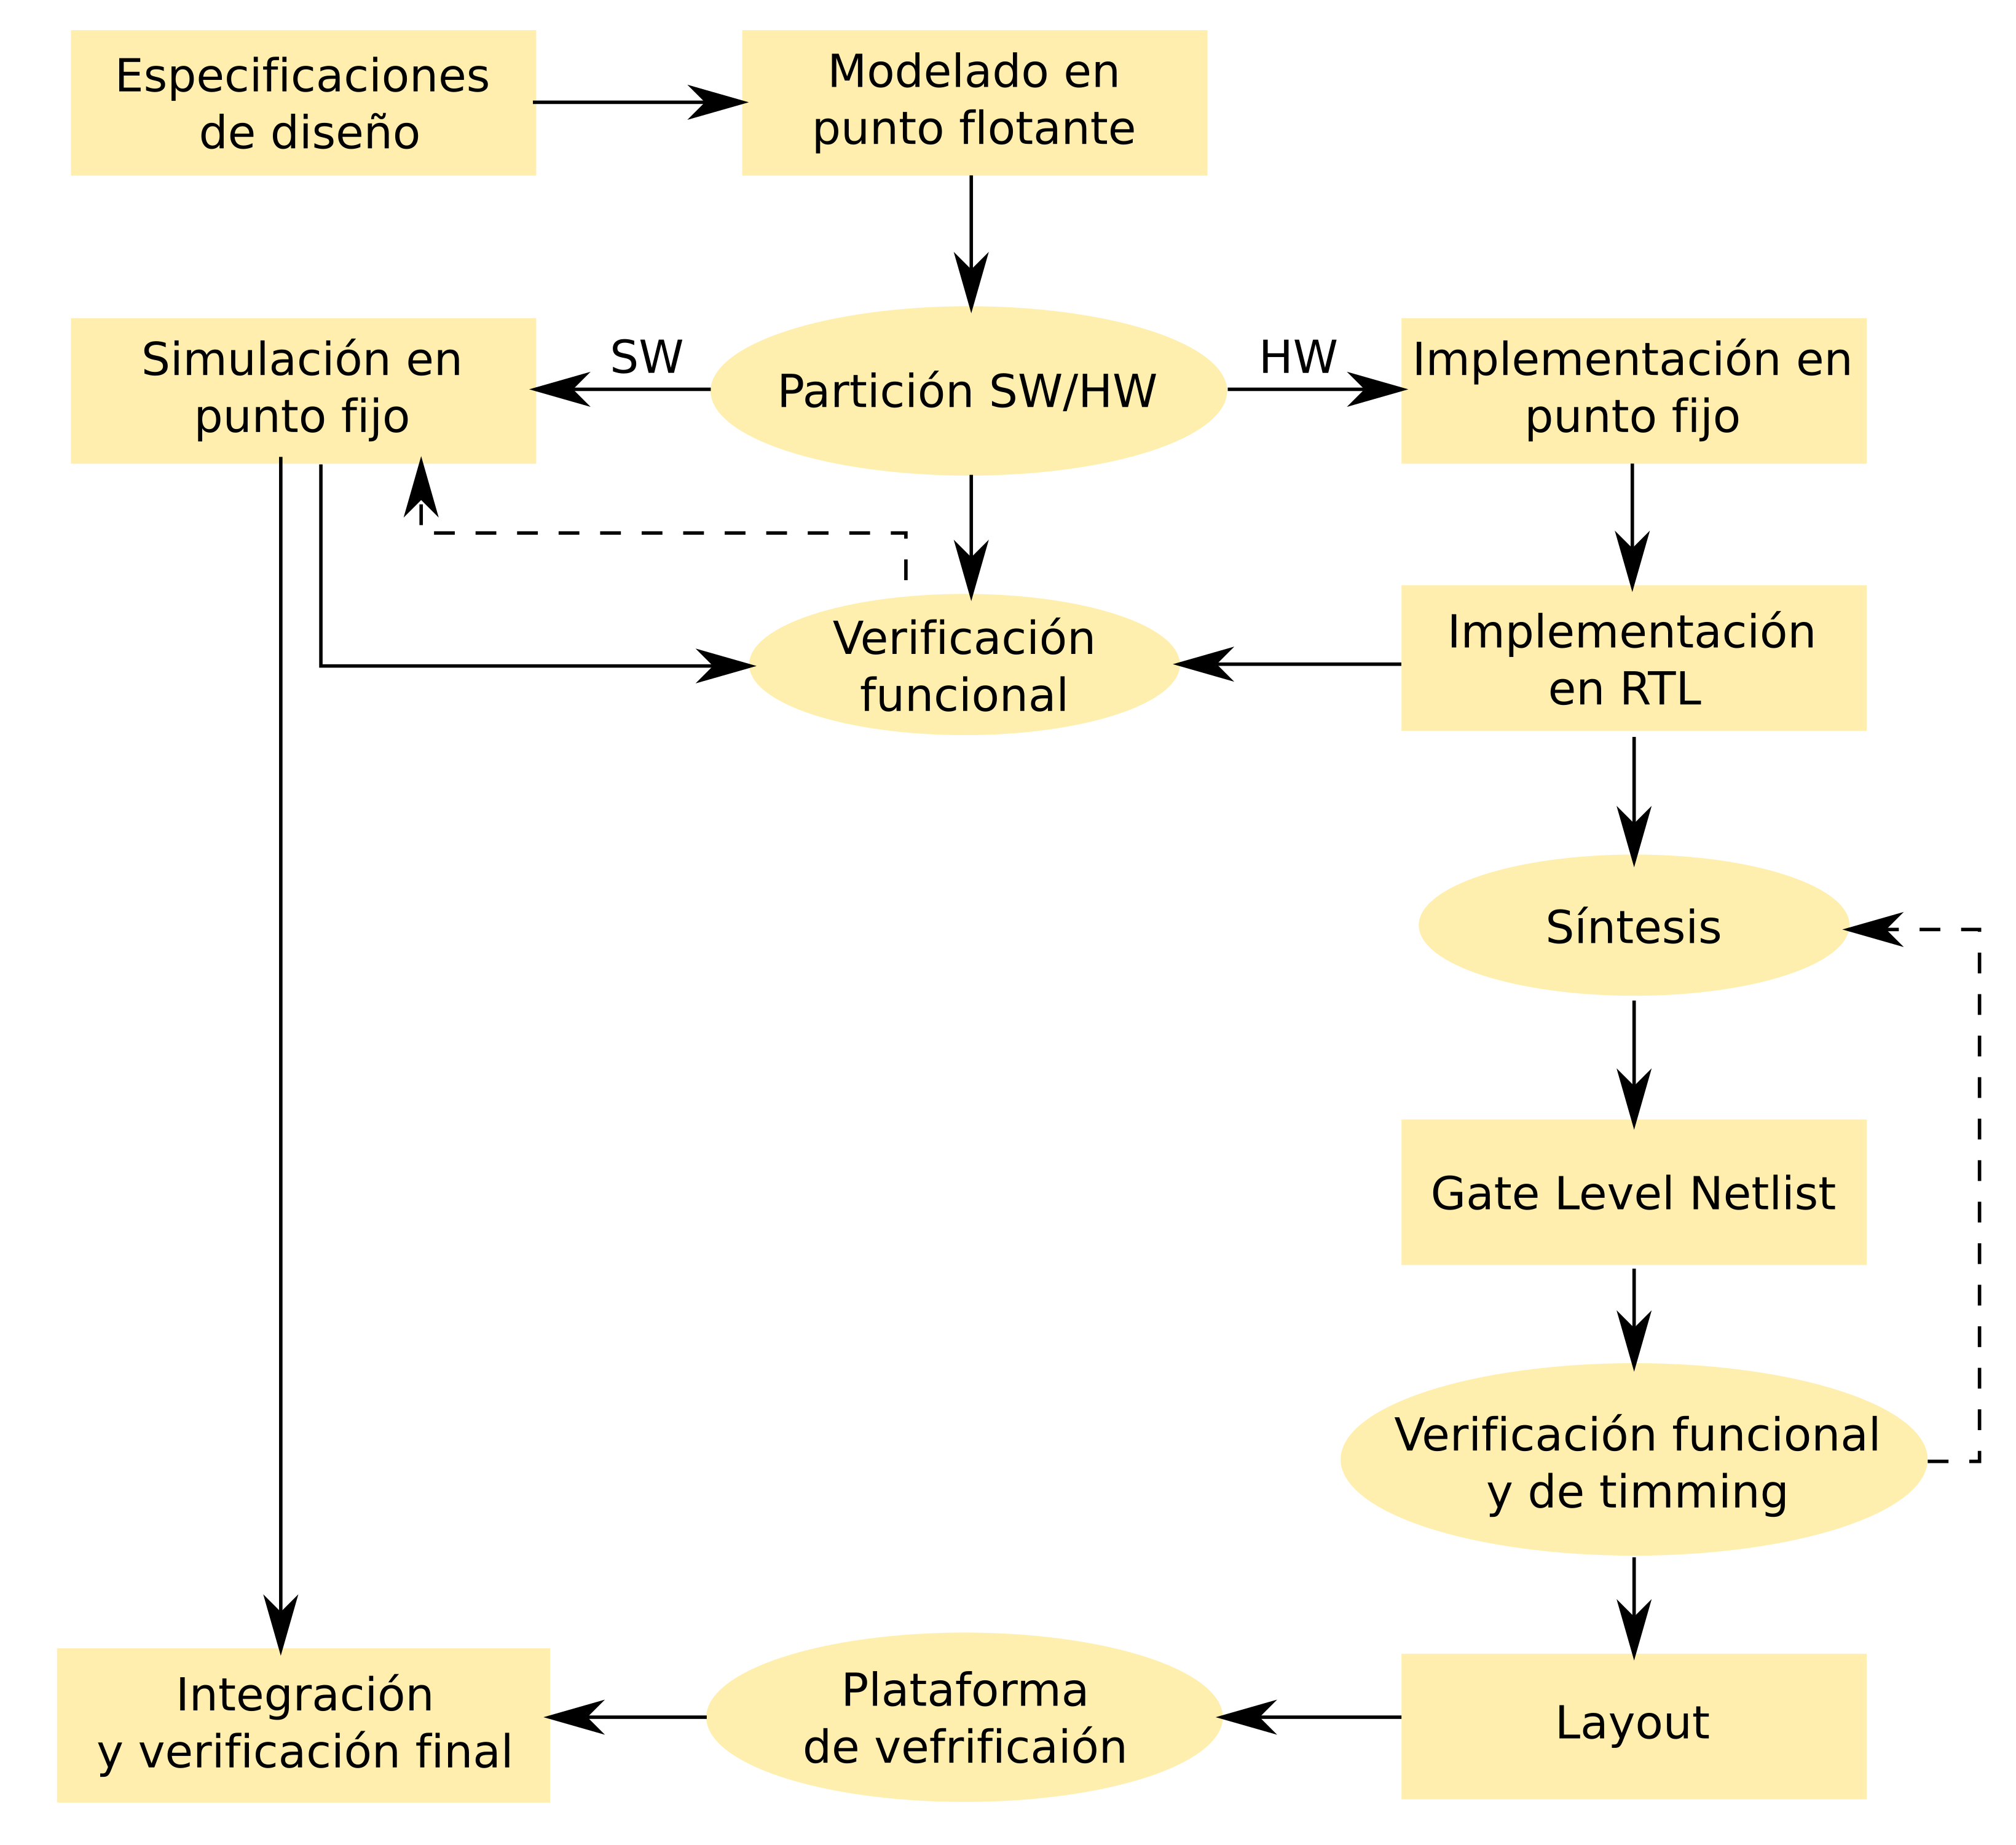
\includegraphics[width=0.65\paperwidth]{Diagramas/diag_flujo.png}
  \end{figure}
\end{frame}



\begin{frame}
  \frametitle{\textbf{Especificaciones y tipos de algoritmos}}
\framesubtitle{\secname : \subsecname}

\begin{block}{\centering \textbf{Especificaciones de diseño}}
    \begin{itemize}\Small
        \item A partir de un DMS con distribución $ P_{(x=0)}= P_{(x=1)}=0.5$ obtener una distribución con una probabilidad de ceros de $P_{(x=0)}= 0.75$.
        \item La secuencia de entrada al codificador deberá ser de 4 bits.
        \item Implementar el mismo con una modulación QAM-16.
    \end{itemize}
\end{block}
\vspace{-0.2cm}
 \begin{block}{\centering \textbf{Tipos de algoritmos}}
     \begin{itemize}\Small
         \item  Según la longitud de la secuencia de datos:
                \begin{itemize}
                     \item Longitud variable a longitud variable (v2v).
                     \item Longitud variable a longitud fija, o viceversa (v2f o f2v).
                     \item Longitud fija a longitud fija (f2f).
                \end{itemize}
        \item   Según el modo de calculo:
                \begin{itemize}
                    \item Online, es decir, en tiempo real.
                    \item Offline, es decir, de forma precalculada.
                \end{itemize}
     \end{itemize}
     
\end{block}

\end{frame}

\begin{frame}
  \frametitle{\textbf{Selección del algoritmo a utilizar}}
     \framesubtitle{\secname : \subsecname}
   
    \begin{block}{\centering \textbf{Algoritmo a utilizar}}
        \begin{itemize}\small
        \item Se utilizará el algoritmo `Constant Composition Distribution Matching' propuesto en \cite{schulte}.
        \item El mismo trabaja con longitudes fijas (f2f) y el calculo es de tipo `online'. 
        % \item Es una técnica de complejidad relativamente baja
        \end{itemize}
    \end{block}
    \vspace{-0.2cm}

    \begin{block}{\centering \textbf{Características del algoritmo}}
        \begin{itemize}\small
            \item Utiliza 'Arithmetic Coding'.
            \item Asocia un intervalo a cada una de las posibles entradas y salidas en base a su probabilidad
            \item Realiza un mapeo de cada intervalo de entrada a un único intervalo de salida
            \item Todas las secuencias de salida tienen una composición constante de `0' y `1'.
        % Insertar imagen intervalos
        \end{itemize}
    \end{block}
\end{frame}


\begin{frame}
  \frametitle{\textbf{Análisis de la longitud de palabra de salida}}
    \framesubtitle{\secname : \subsecname}
   \begin{block}{\centering \textbf{Longitud de palabra de salida}}
        \begin{itemize}\footnotesize
            \item  Cantidad de bits de entrada
            \item La probabilidad $P_{(x=1)}$ deseada
        \end{itemize}
    \end{block}
    \vspace{-0.2cm}

    \begin{block}{\centering \textbf{Condiciones necesarias}}
        \begin{itemize}\footnotesize
            \item Se debe cumplir que:
            \begin{equation*}
            {X \choose Y} \geq 2^{k}    
            \end{equation*}
        \item Donde:
            \begin{itemize}\footnotesize
                \item [$X$:] Longitud de secuencia de salida.
                \item [$Y$:] Cantidad de bits de salida en `1'.
                \item [$k$:] Longitud de secuencia entrada. 
            \end{itemize}
        \item Además se debe mantener la relación:
            \begin{equation*}
            \frac{X}{Y} =  \frac{1}{P_{(x=1)}}  
            \end{equation*}
        \end{itemize}
    \end{block}

\end{frame}

\begin{frame}
  \frametitle{\textbf{Análisis de la longitud de palabra de salida}}
    %  \framesubtitle{\secname : \subsecname}
    \begin{block}{\centering \textbf{Longitud de salida las para especificaciones de diseño}}
    \begin{itemize}\Small
        \item Para $k=4$ y $P_{(x=1)} = 0.25$ tendremos:
            \begin{equation*}
            \frac{X}{Y} = \frac{1}{P_{(x=1)}} = 4 \implies X = 4*Y
            \end{equation*}
        \item A su vez:
            \begin{equation*} 
            {X \choose Y} \geq 16 \implies X=8 \implies \frac{X-k}{k} = 100\% 
            \end{equation*}
    \end{itemize}
    \end{block}
        \begin{block}{\centering \textbf{Ejemplos para otras especificaciones}}
        \begin{itemize}
        \item $k=16$ y $P_{(x=1)} = 0.25 \implies {24 \choose 6} \geq 2^{16} \implies \frac{X-k}{k} = 50\%$ 
        \item  $k=4$ y $P_{(x=1)} = 0.285 \implies {7 \choose 2} \geq 2^{4} \implies \frac{X-k}{k} = 75\%$
    \end{itemize}
    \end{block}
\end{frame}



\begin{frame}
  \frametitle{\textbf{Calculo de intervalo de entrada del  codificador}}
\framesubtitle{\secname : \subsecname}
   \begin{block}{Ejemplo}
   \begin{itemize}
    \item $Xi_{cod} = 1010$ y $P_{(x=0)}=0.75$: 
  \end{itemize}
  \end{block}
      \vspace{-0.3cm}
  \begin{figure}[!t] \centering
  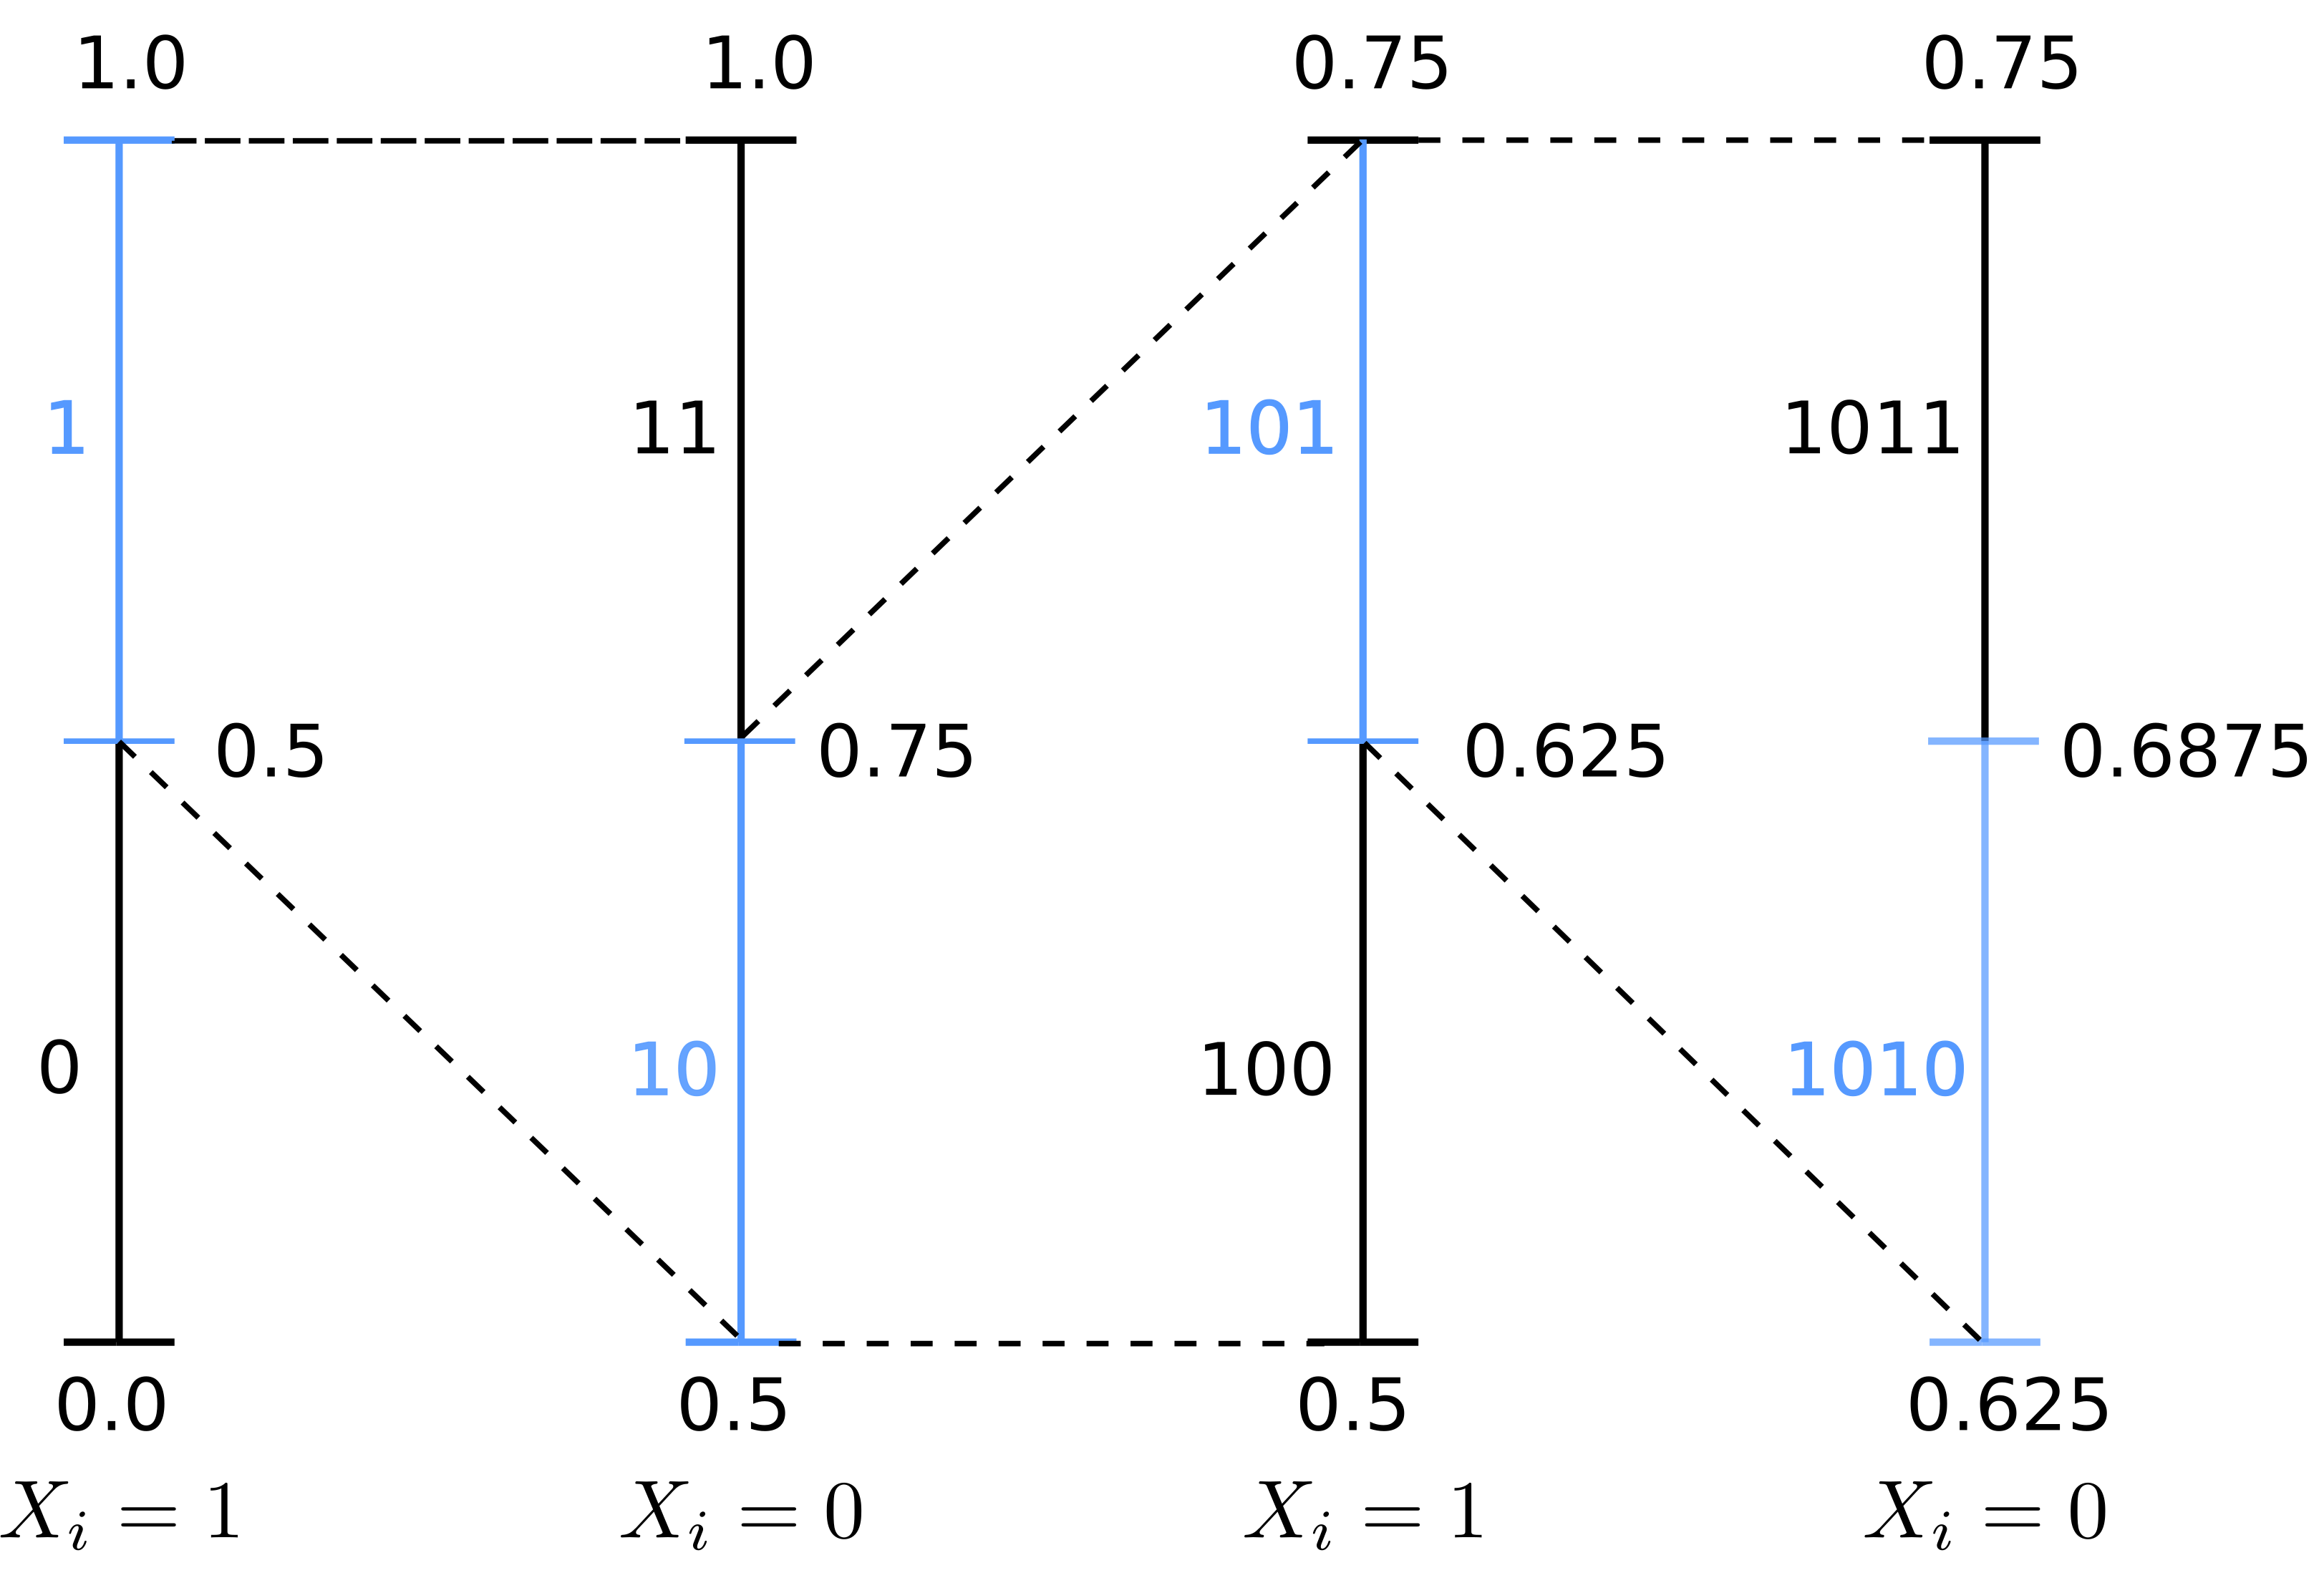
\includegraphics[width=0.80\paperheight]{Diagramas/int_ent_cod.png}%
  \end{figure}
\end{frame}

\begin{frame}
  \frametitle{\textbf{Intervalo de salida del bloque codificador}}
\framesubtitle{\secname : \subsecname}
   \begin{block}{\centering \textbf{Concepto de `Bolsa de bits'}}
   \begin{itemize}
    \item Propuesto en \cite[Sec.\ 4]{schulte}.
    \item En cada iteración se elimina un bit, obteniendo una nueva probabilidad. $P_{(x=0)}$ 
    \end{itemize}
  \end{block}
      \vspace{-0.3cm}
  \begin{figure}[!t] \centering
  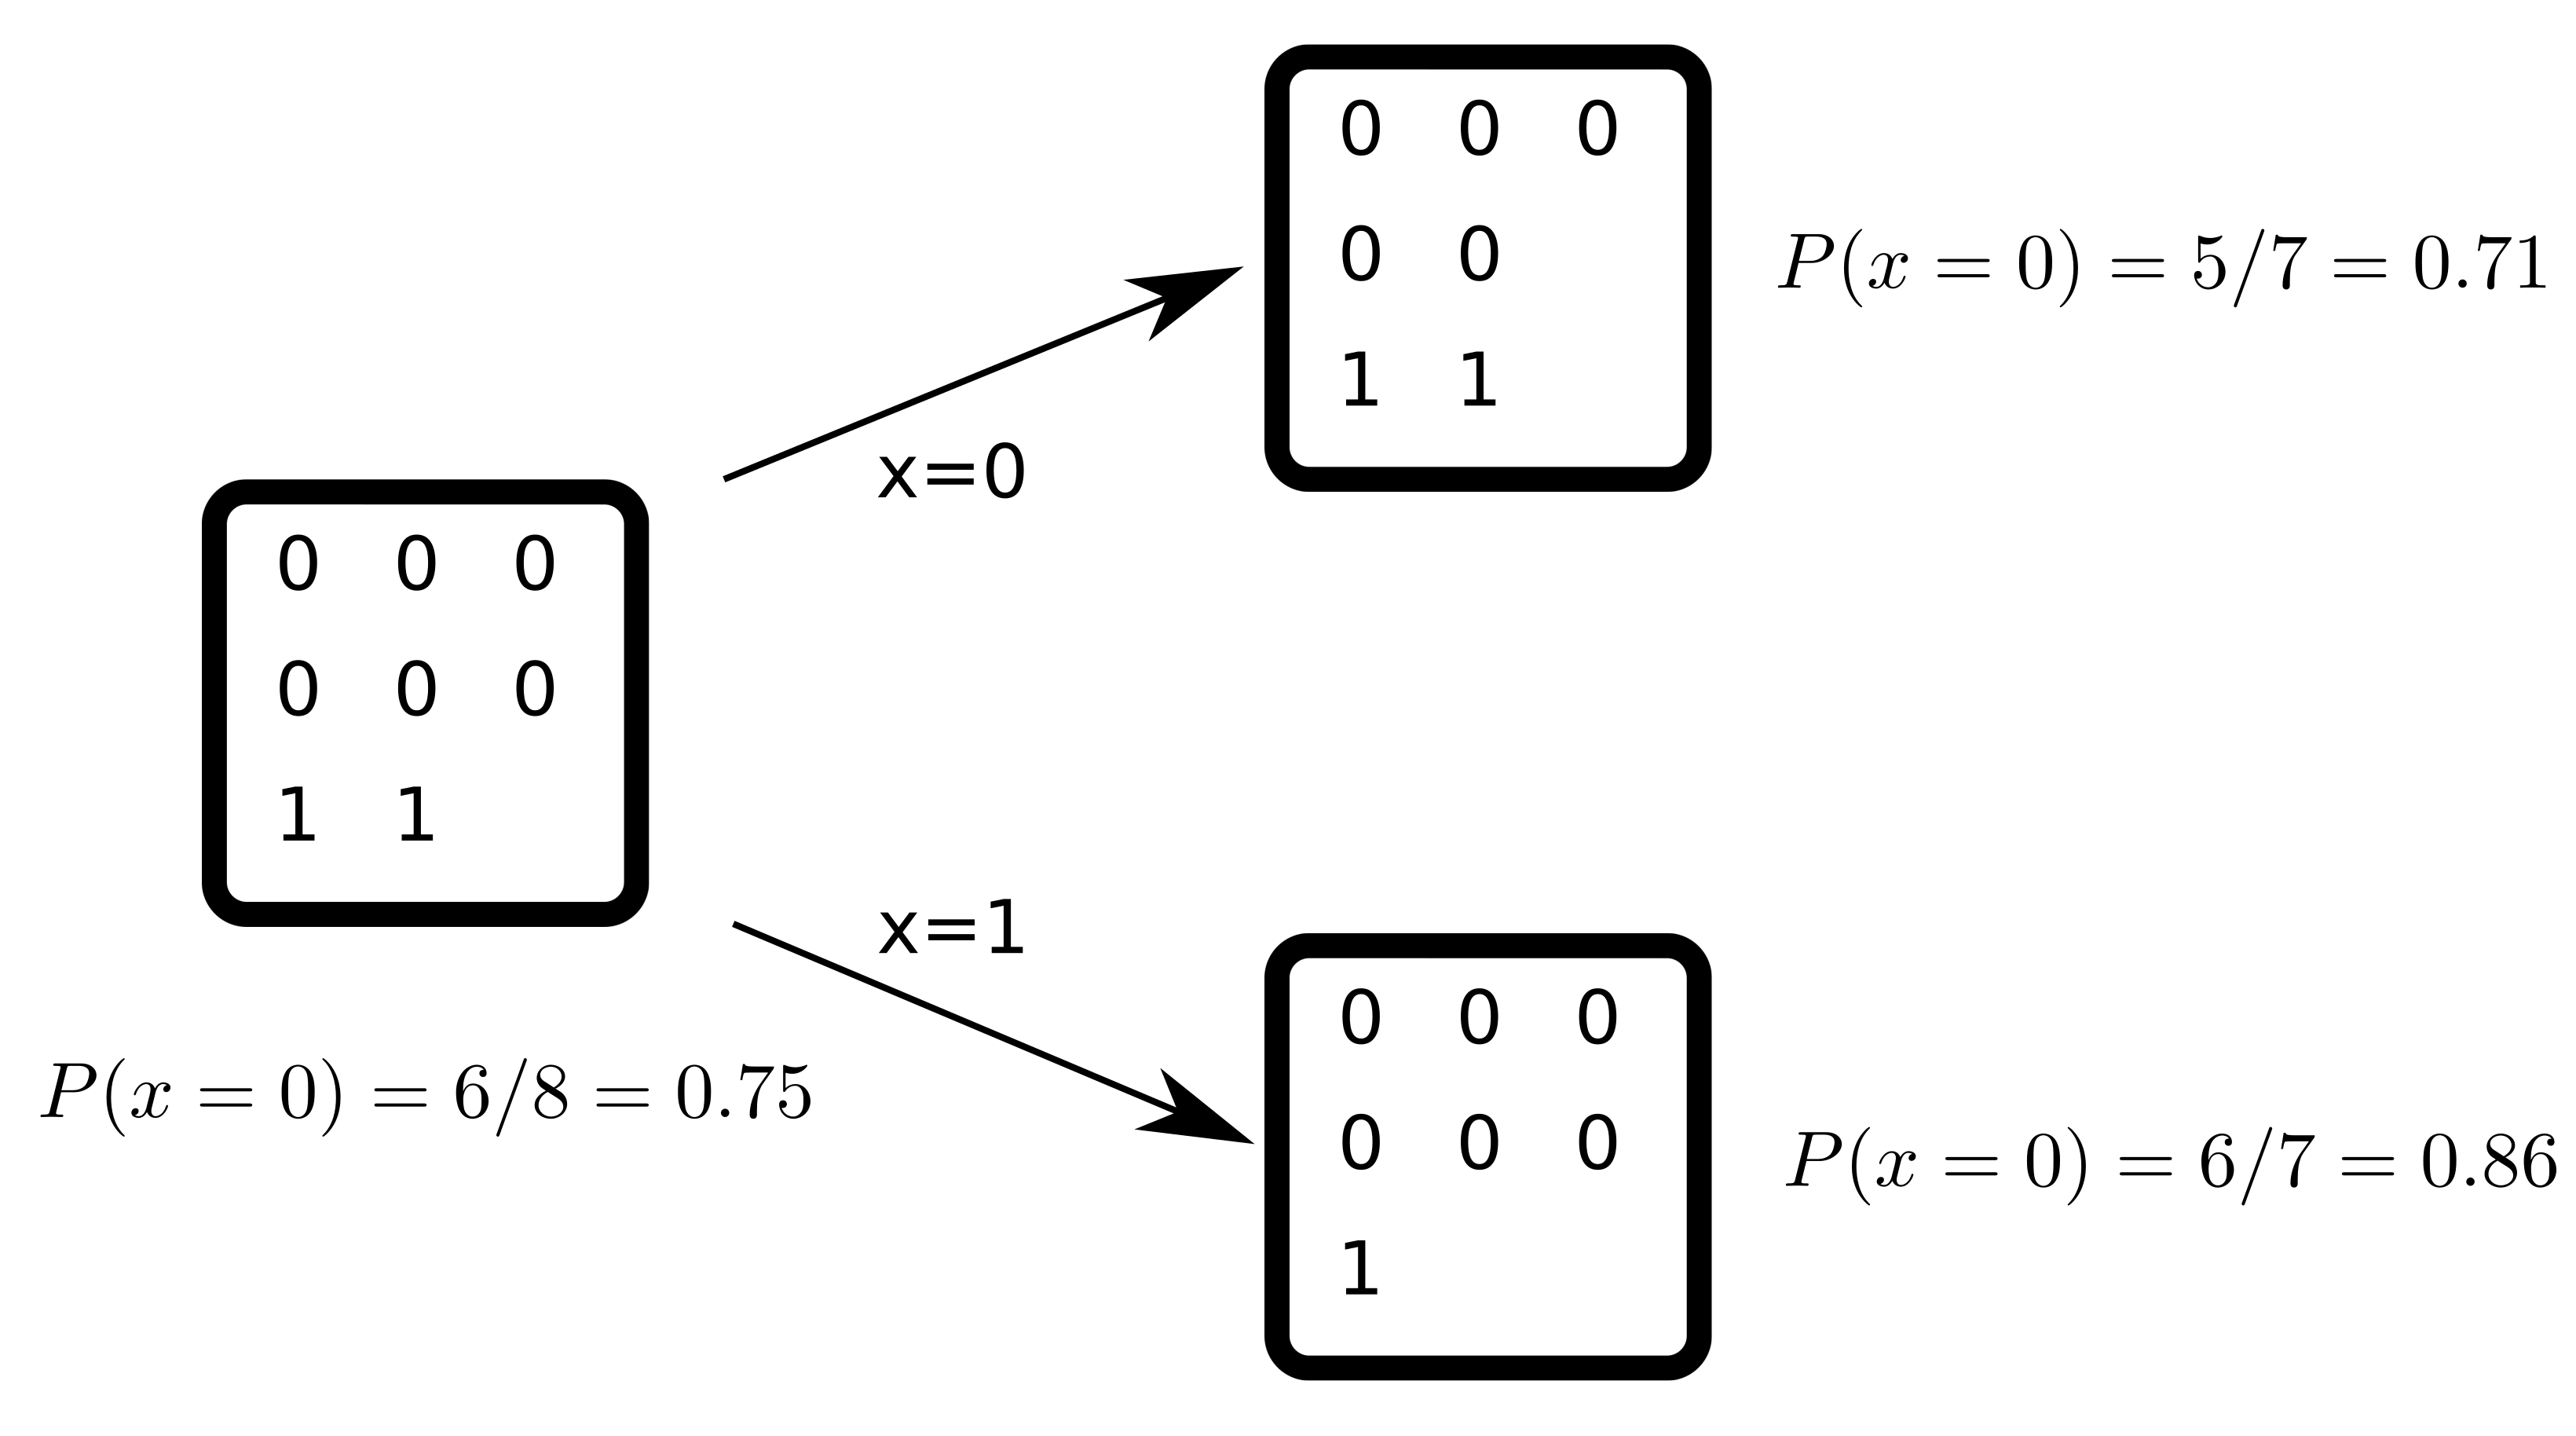
\includegraphics[width=0.70\paperwidth]{Diagramas/bag.png}%
  \end{figure}
\end{frame}

\begin{frame}
  \frametitle{\textbf{Calculo de Intervalo de salida del  codificador}}
\framesubtitle{\secname : \subsecname}
   \begin{block}{\centering \textbf{Concepto de `Escalado'}}
       \begin{itemize}\Small
            \item Propuesto en \cite[Sec.\ 4]{schulte}.
            \item Permite aumentar los límites de los subintervalos cuando estos cumplen con las siguientes condiciones:
            \begin{itemize}\footnotesize
                \item Si $u_s \leq 0.5$:
                    \begin{itemize}
                        \item $u_s' = 2  u_s$
                        \item $l_s' = 2 l_s$
                        \item $l_i' = 2  l_i$
                    \end{itemize}
                \item Si $l_s > 0.5$: 
                    \begin{itemize}
                        \item $u_s' = 2  (u_s - 0.5)$
                        \item $l_s' = 2  (l_s - 0.5)$
                        \item $l_i' = 2  (l_i - 0.5)$
                    \end{itemize}
            \end{itemize}
            \item Esto permitirá optimizar la cantidad de bits en la implementación.
        \end{itemize}
  \end{block}
\end{frame}


\begin{frame}
  \frametitle{\textbf{Calculo de intervalo de salida del bloque codificador}}
\framesubtitle{\secname : \subsecname}
   \begin{block}{Ejemplo}
   \begin{itemize}
    \item $Xi_{cod} = 1010$ y $P_{(x=0)}=0.75$: 
  \end{itemize}
  \end{block}
      \vspace{-0.3cm}
  \begin{figure}[!t] \centering
  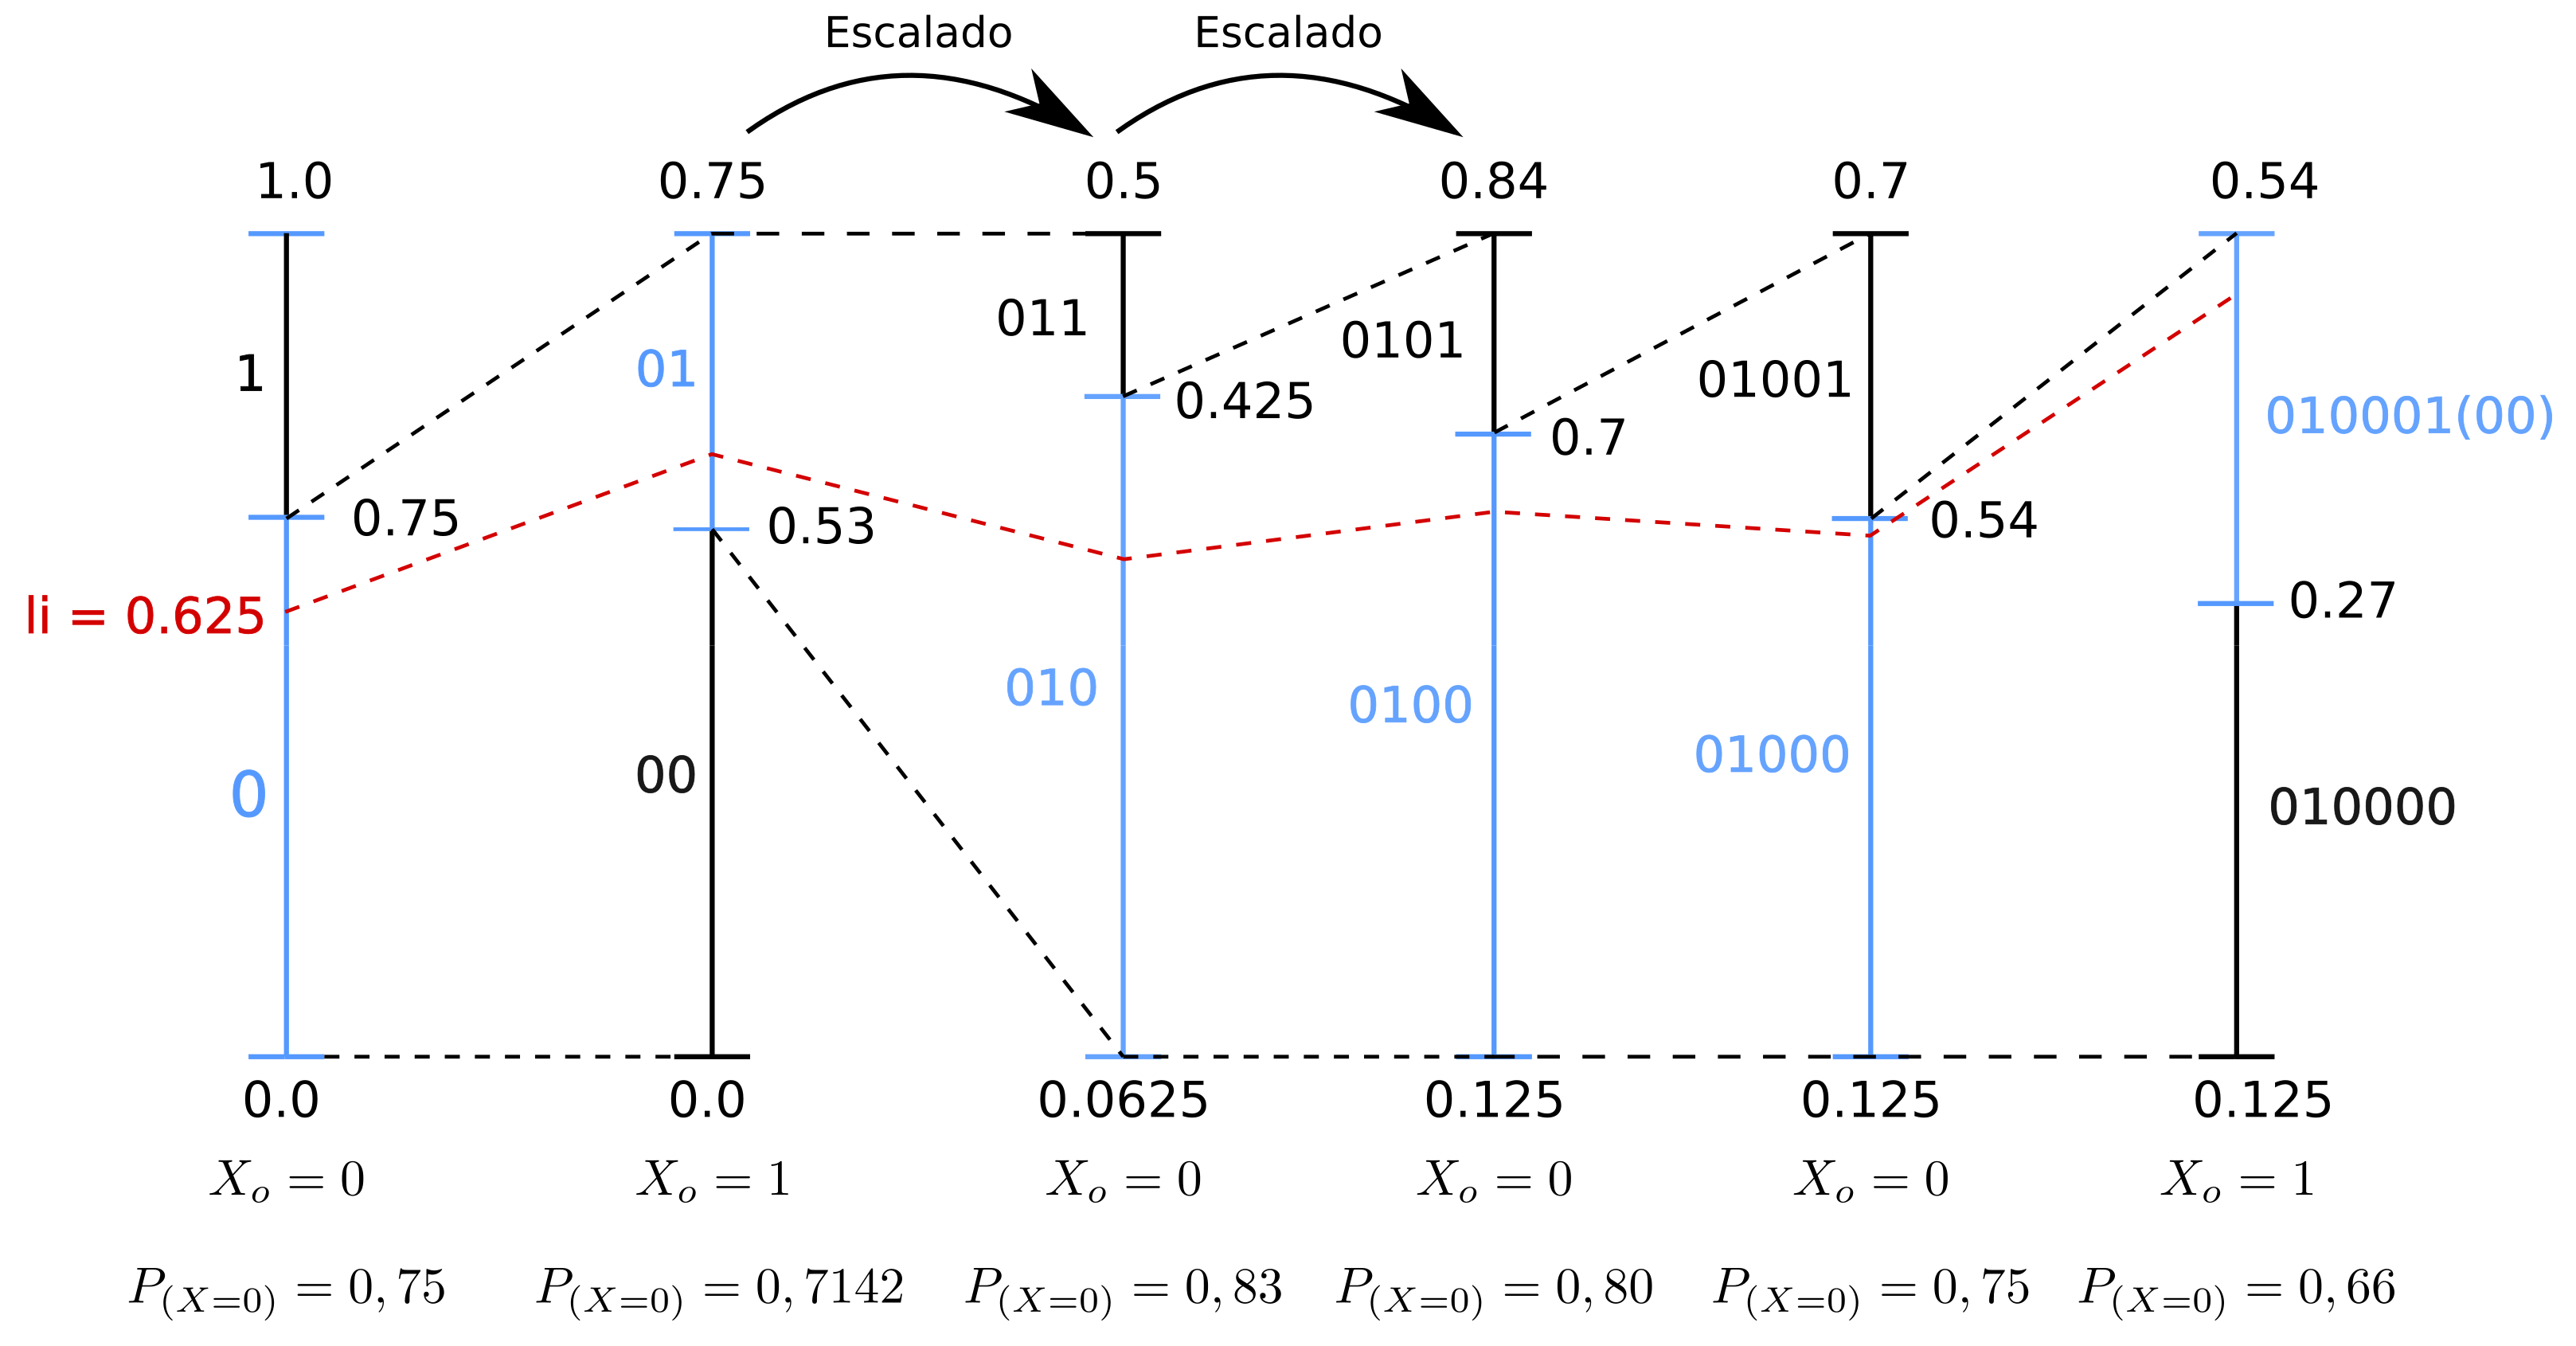
\includegraphics[width=0.85\paperwidth]{Diagramas/int_sal_cod.png}%
  \end{figure}
\end{frame}


\begin{frame}
  \frametitle{\textbf{Calculo de intervalo de entrada del  decodificador}}
\framesubtitle{\secname : \subsecname}
   \begin{block}{Ejemplo}
   \begin{itemize}
    \item $Xi_{cod} = 01000100$ y  $P_{(x=0)}=0.75$:
  \end{itemize}
  \end{block}
      \vspace{-0.3cm}
  \begin{figure}[!t] \centering
  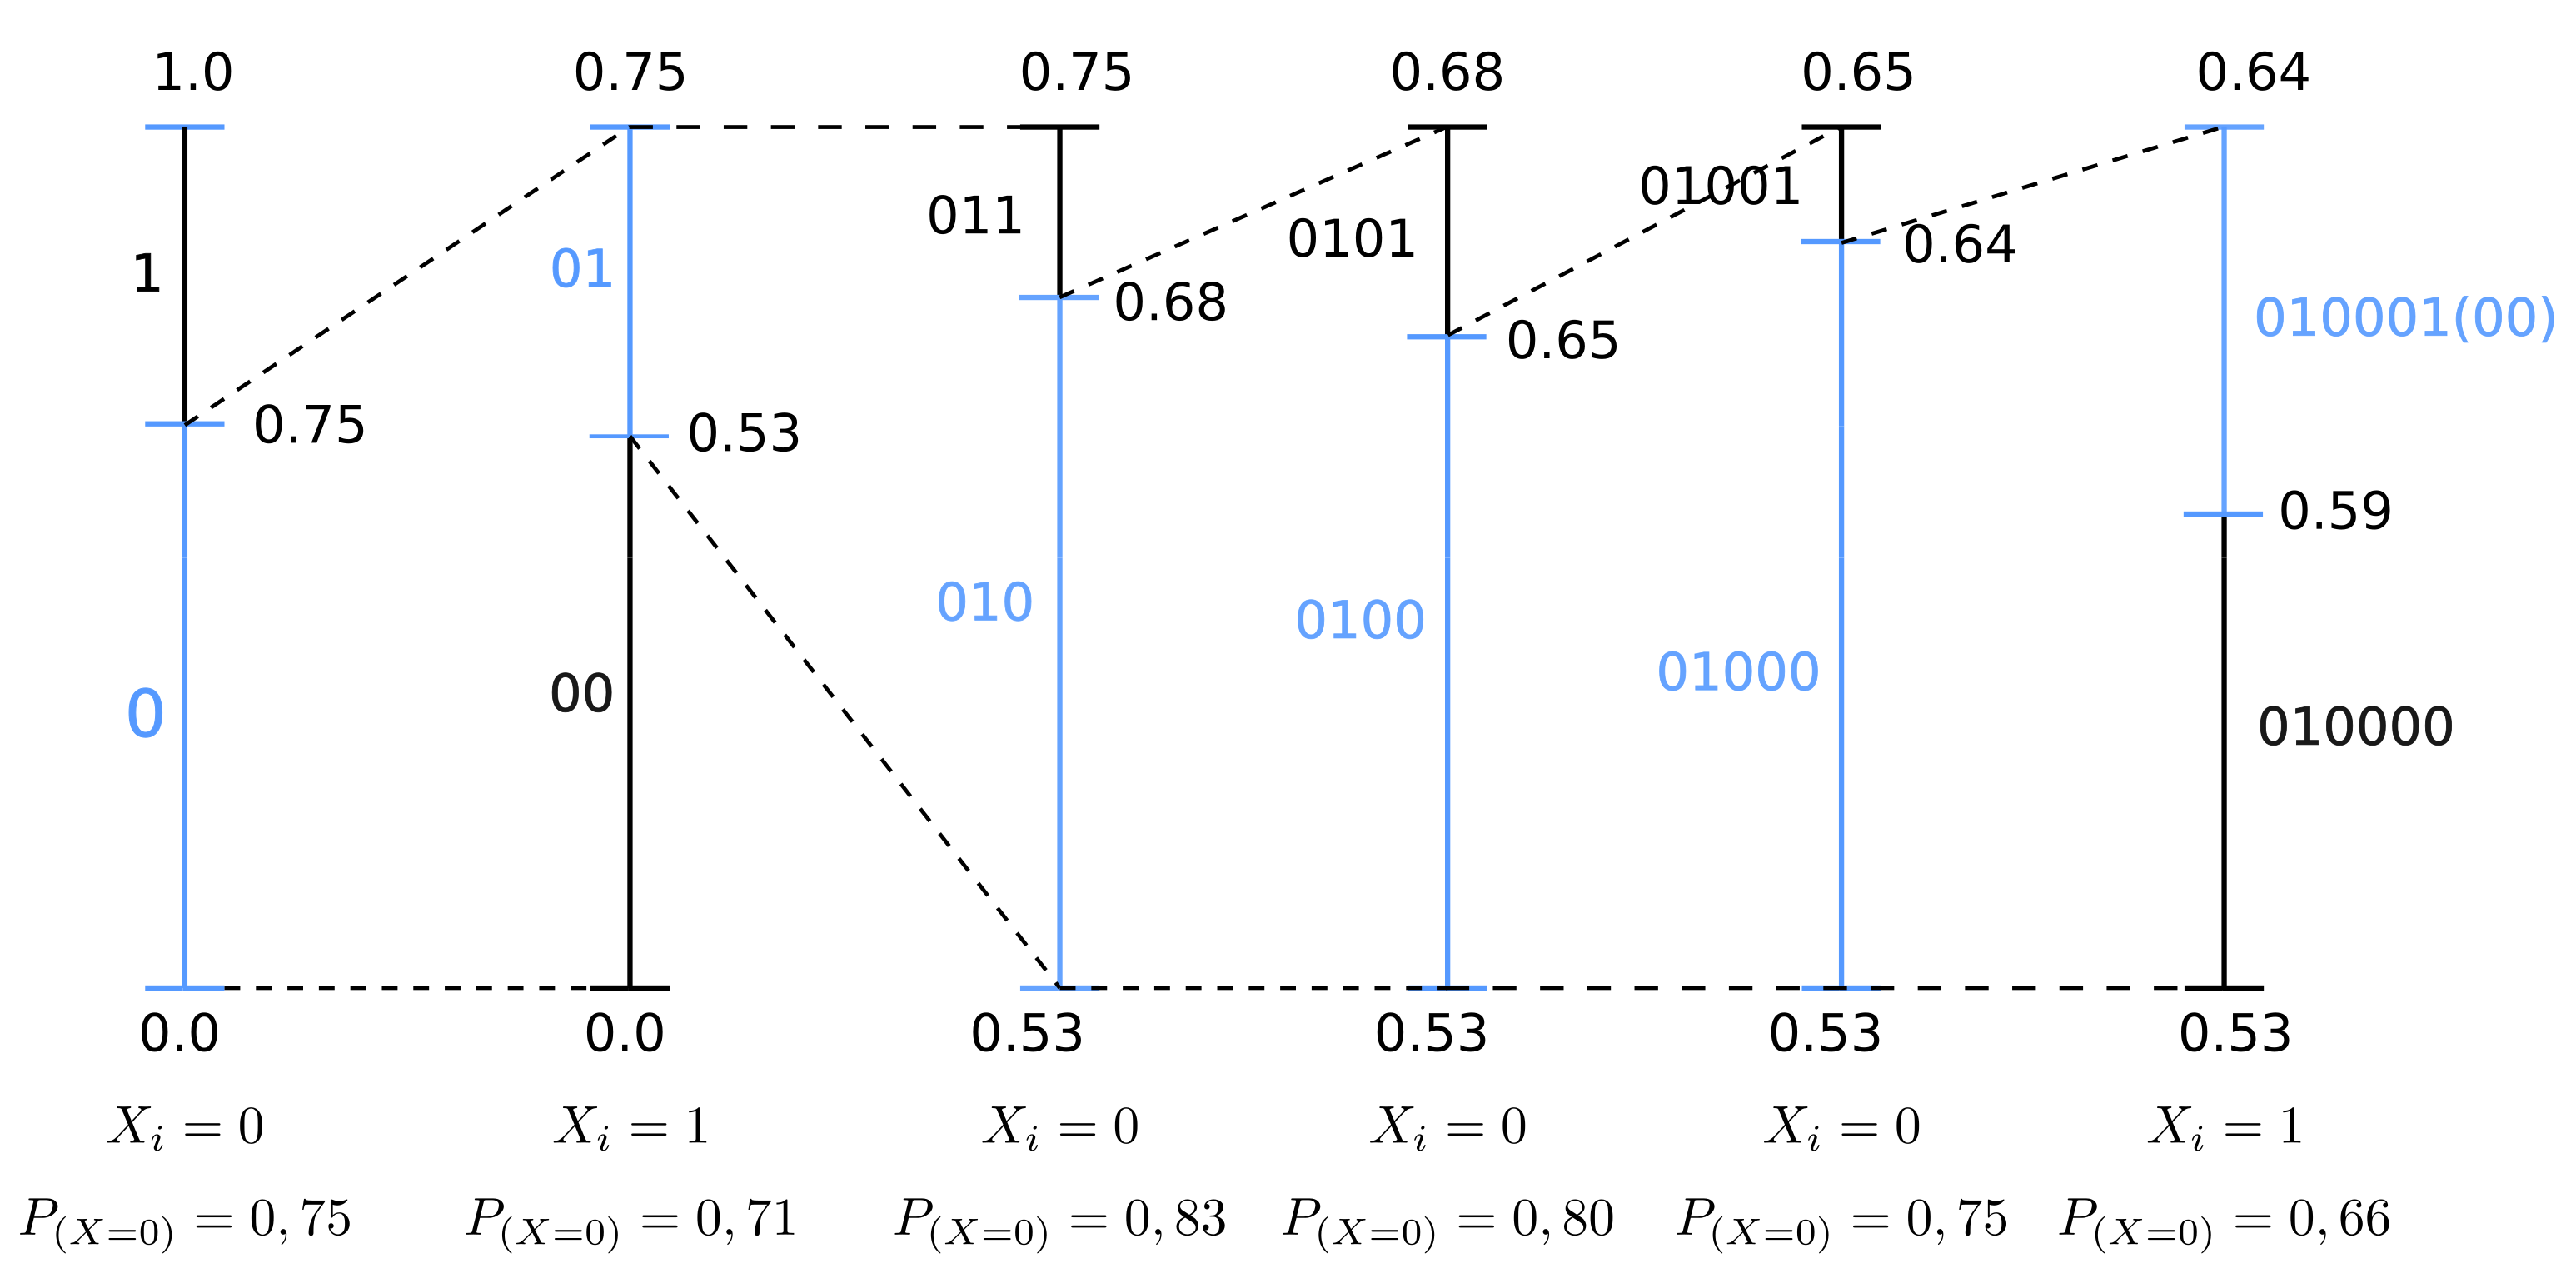
\includegraphics[width=0.85\paperwidth]{Diagramas/int_ent_dec.png}%
  \end{figure}
\end{frame}

\begin{frame}
  \frametitle{\textbf{Calculo de intervalo de salida del  decodificador}}
\framesubtitle{\secname : \subsecname}
   \begin{block}{Ejemplo}
   \begin{itemize}
    \item $Xi_{cod} = 01000100$ y  $P_{(x=0)}=0.75$:
  \end{itemize}
  \end{block}
      \vspace{-0.3cm}
  \begin{figure}[!t] \centering
  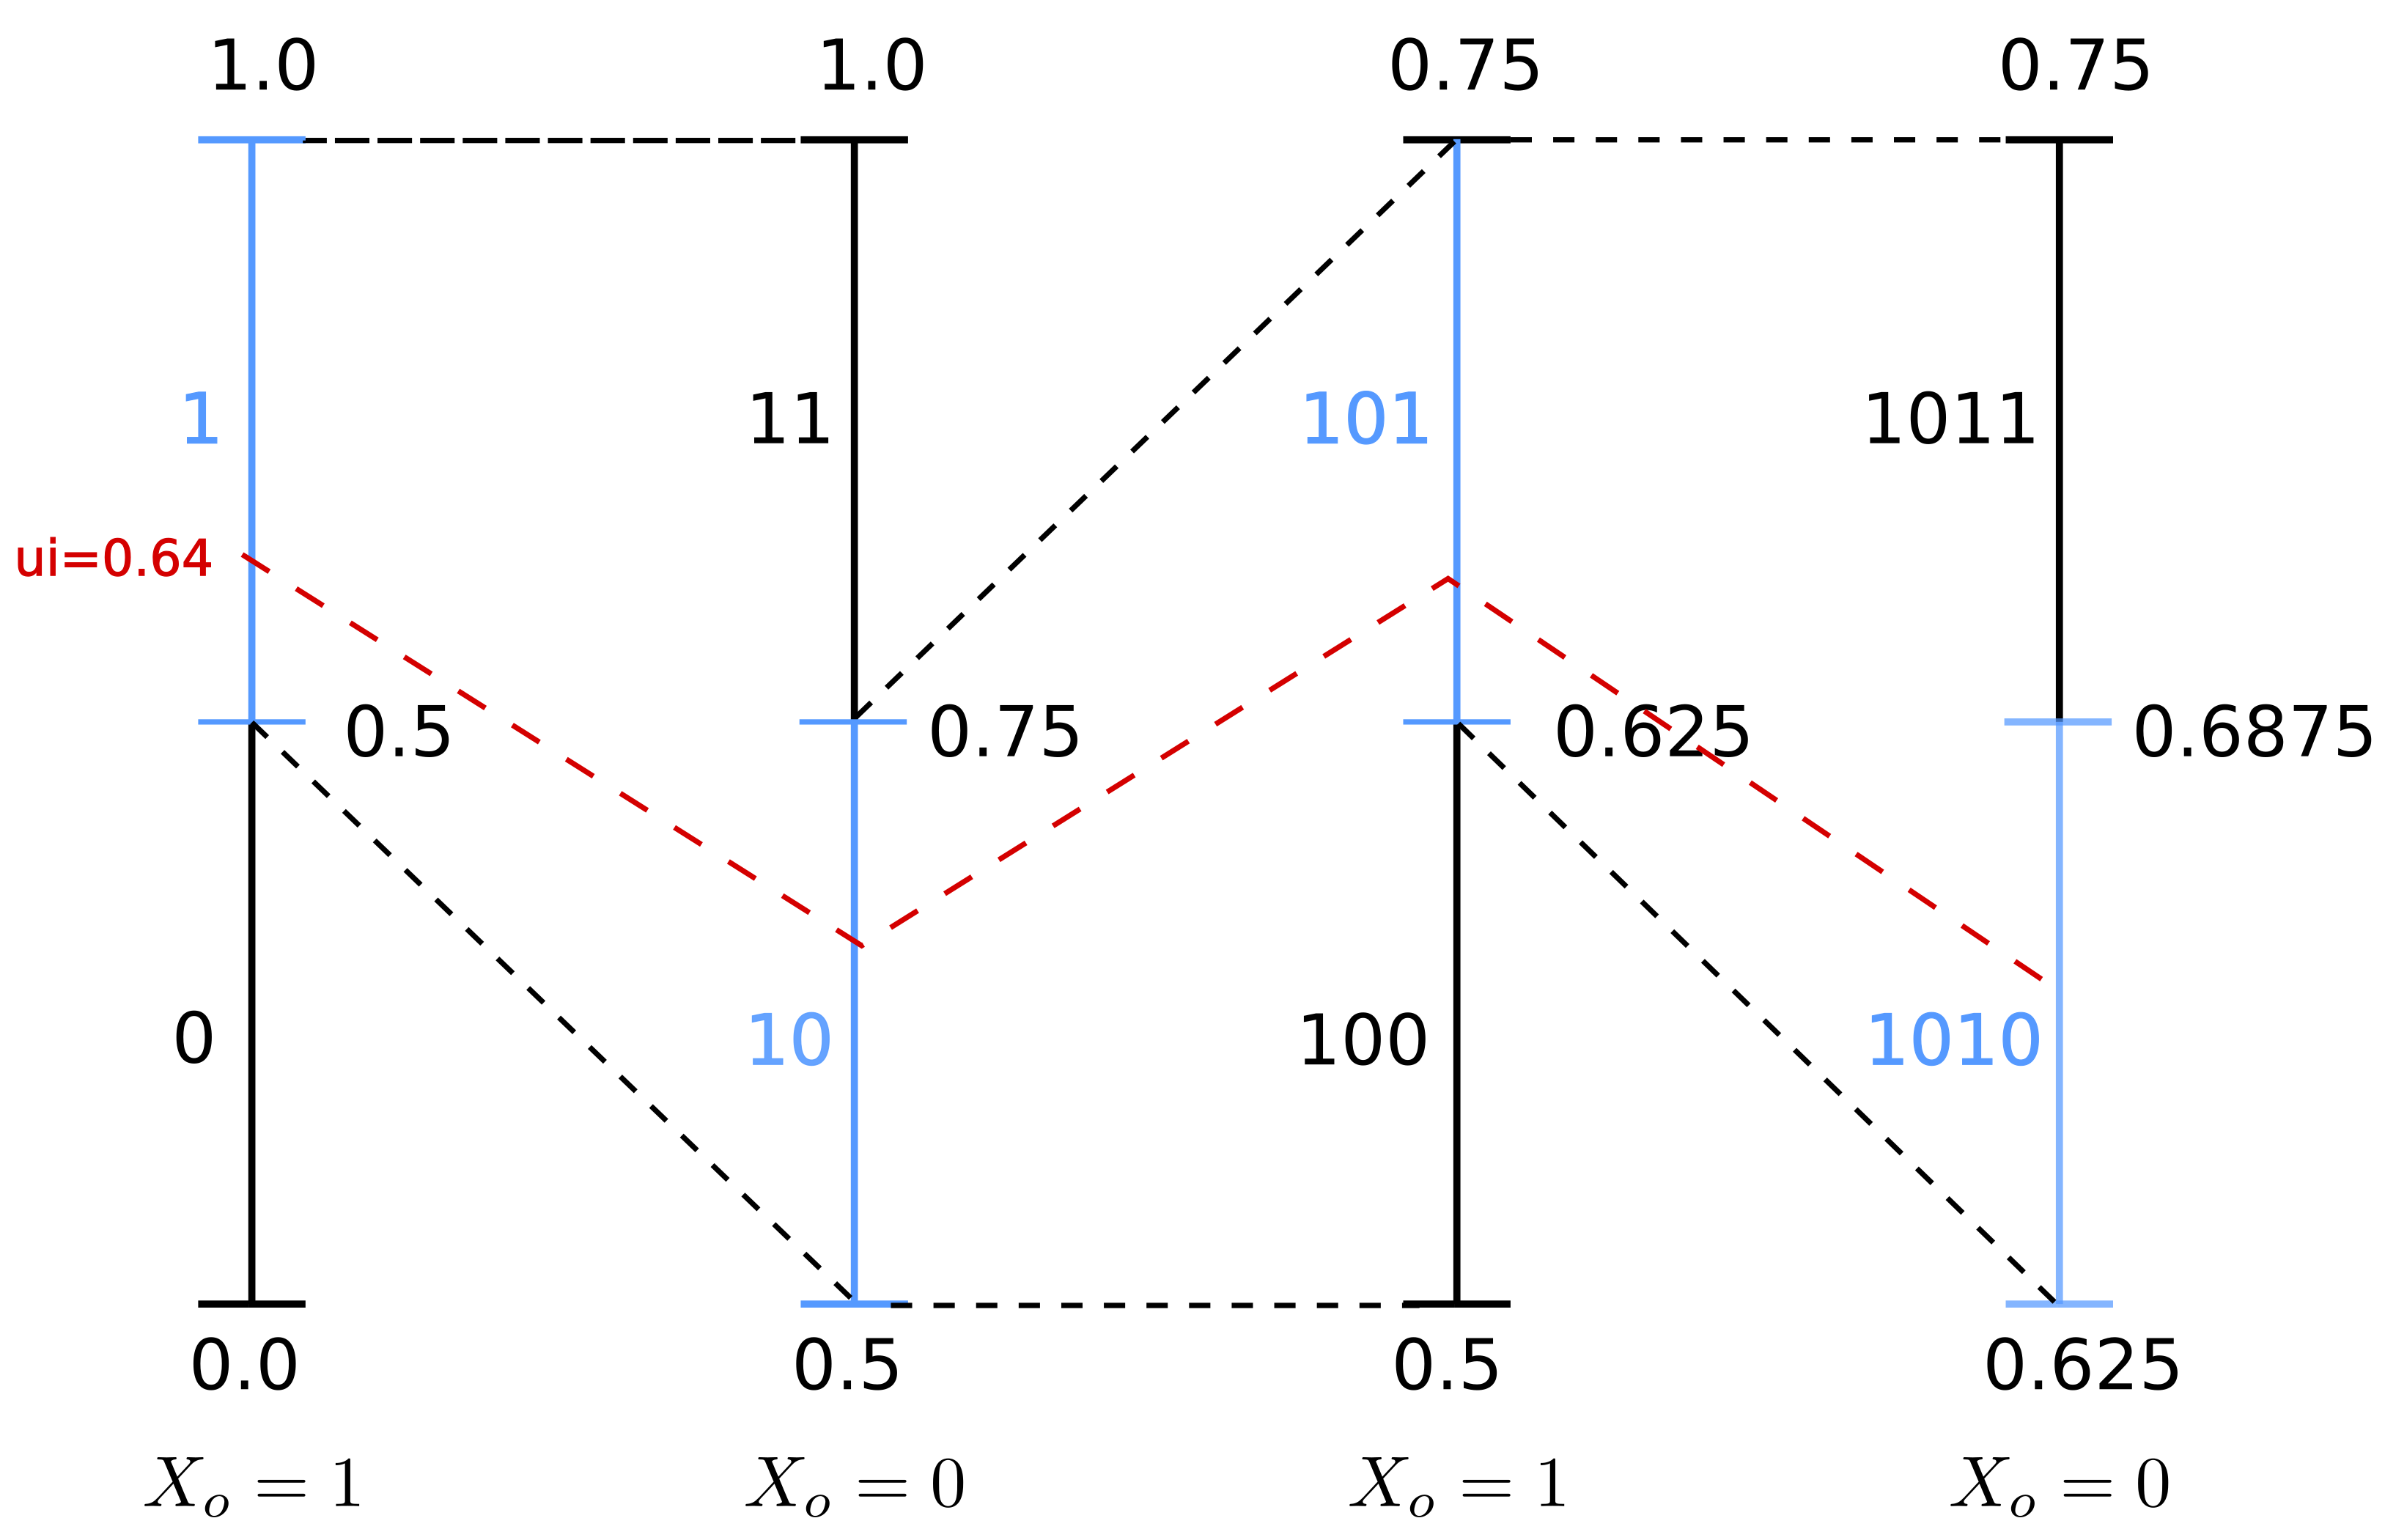
\includegraphics[width=0.70\paperwidth]{Diagramas/int_sal_dec.png}%
  \end{figure}
\end{frame}



